\section{Implementation}
The implementation process involves the following steps
\begin{itemize}
	\item Taking the driver code and integrating it with a Linux kernel using Buildroot. This steps involves copying the drivers files into the right directories and then making changes to the kernel Makefiles and KConfig files in order for the kernel menu menuconfig to reflect on these changes. Once the changes are made, it is essential to enable them in the kernel menu using the following command in Buildroot:
	\begin{center}
		\textbf{make linux-menuconfig}\\
	\end{center}
	This will open the configuration menu for the kernel. The spi driver is to be enabled after browsing into \textbf{Drivers: Bluetooth}.
	\begin{figure}[ht]
		\centering
		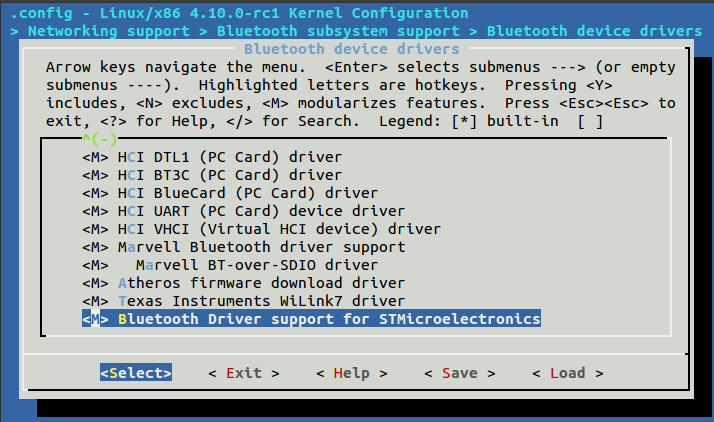
\includegraphics[width=3.5in, height=3in]{images/menu_implementation.png}
		\caption{The DTS entry}
	\end{figure}
	\item Making changes in the DTS file is very important. Without doing this, the driver code will not work as the Linux kernel will have no way of connecting the driver code to the hardware. The changes are made in the DTS file and the file is compiled into a DTB file. This DTB file is used when the kernel boots to connect all the hardware to the right piece of software. The DTS file for Raspberry Pi 3 model is \textbf{bcm-2710-rpi-3-b.dts}
	\begin{figure}[ht]
		\centering
		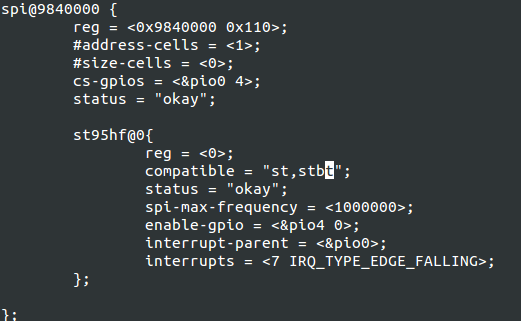
\includegraphics[width=3.5in, height=3in]{images/dts_implementation.png}
		\caption{The DTS entry}
	\end{figure}
	\item After the entry in the DTS, it is time to make the connection between the board and the BlueNRG chip. The following lines are to connected for a successful SPI transaction.
	\begin{enumerate}
		\item \textbf{MISO}
		\item \textbf{MOSI}
		\item \textbf{CS}
		\item \textbf{SCLK}
		\item \textbf{INR}
	\end{enumerate}
	Make these changes according to the pin layout of the board and the BlueNRG. Following pictures shows the connections made.
	\begin{figure}[ht]
		\centering
		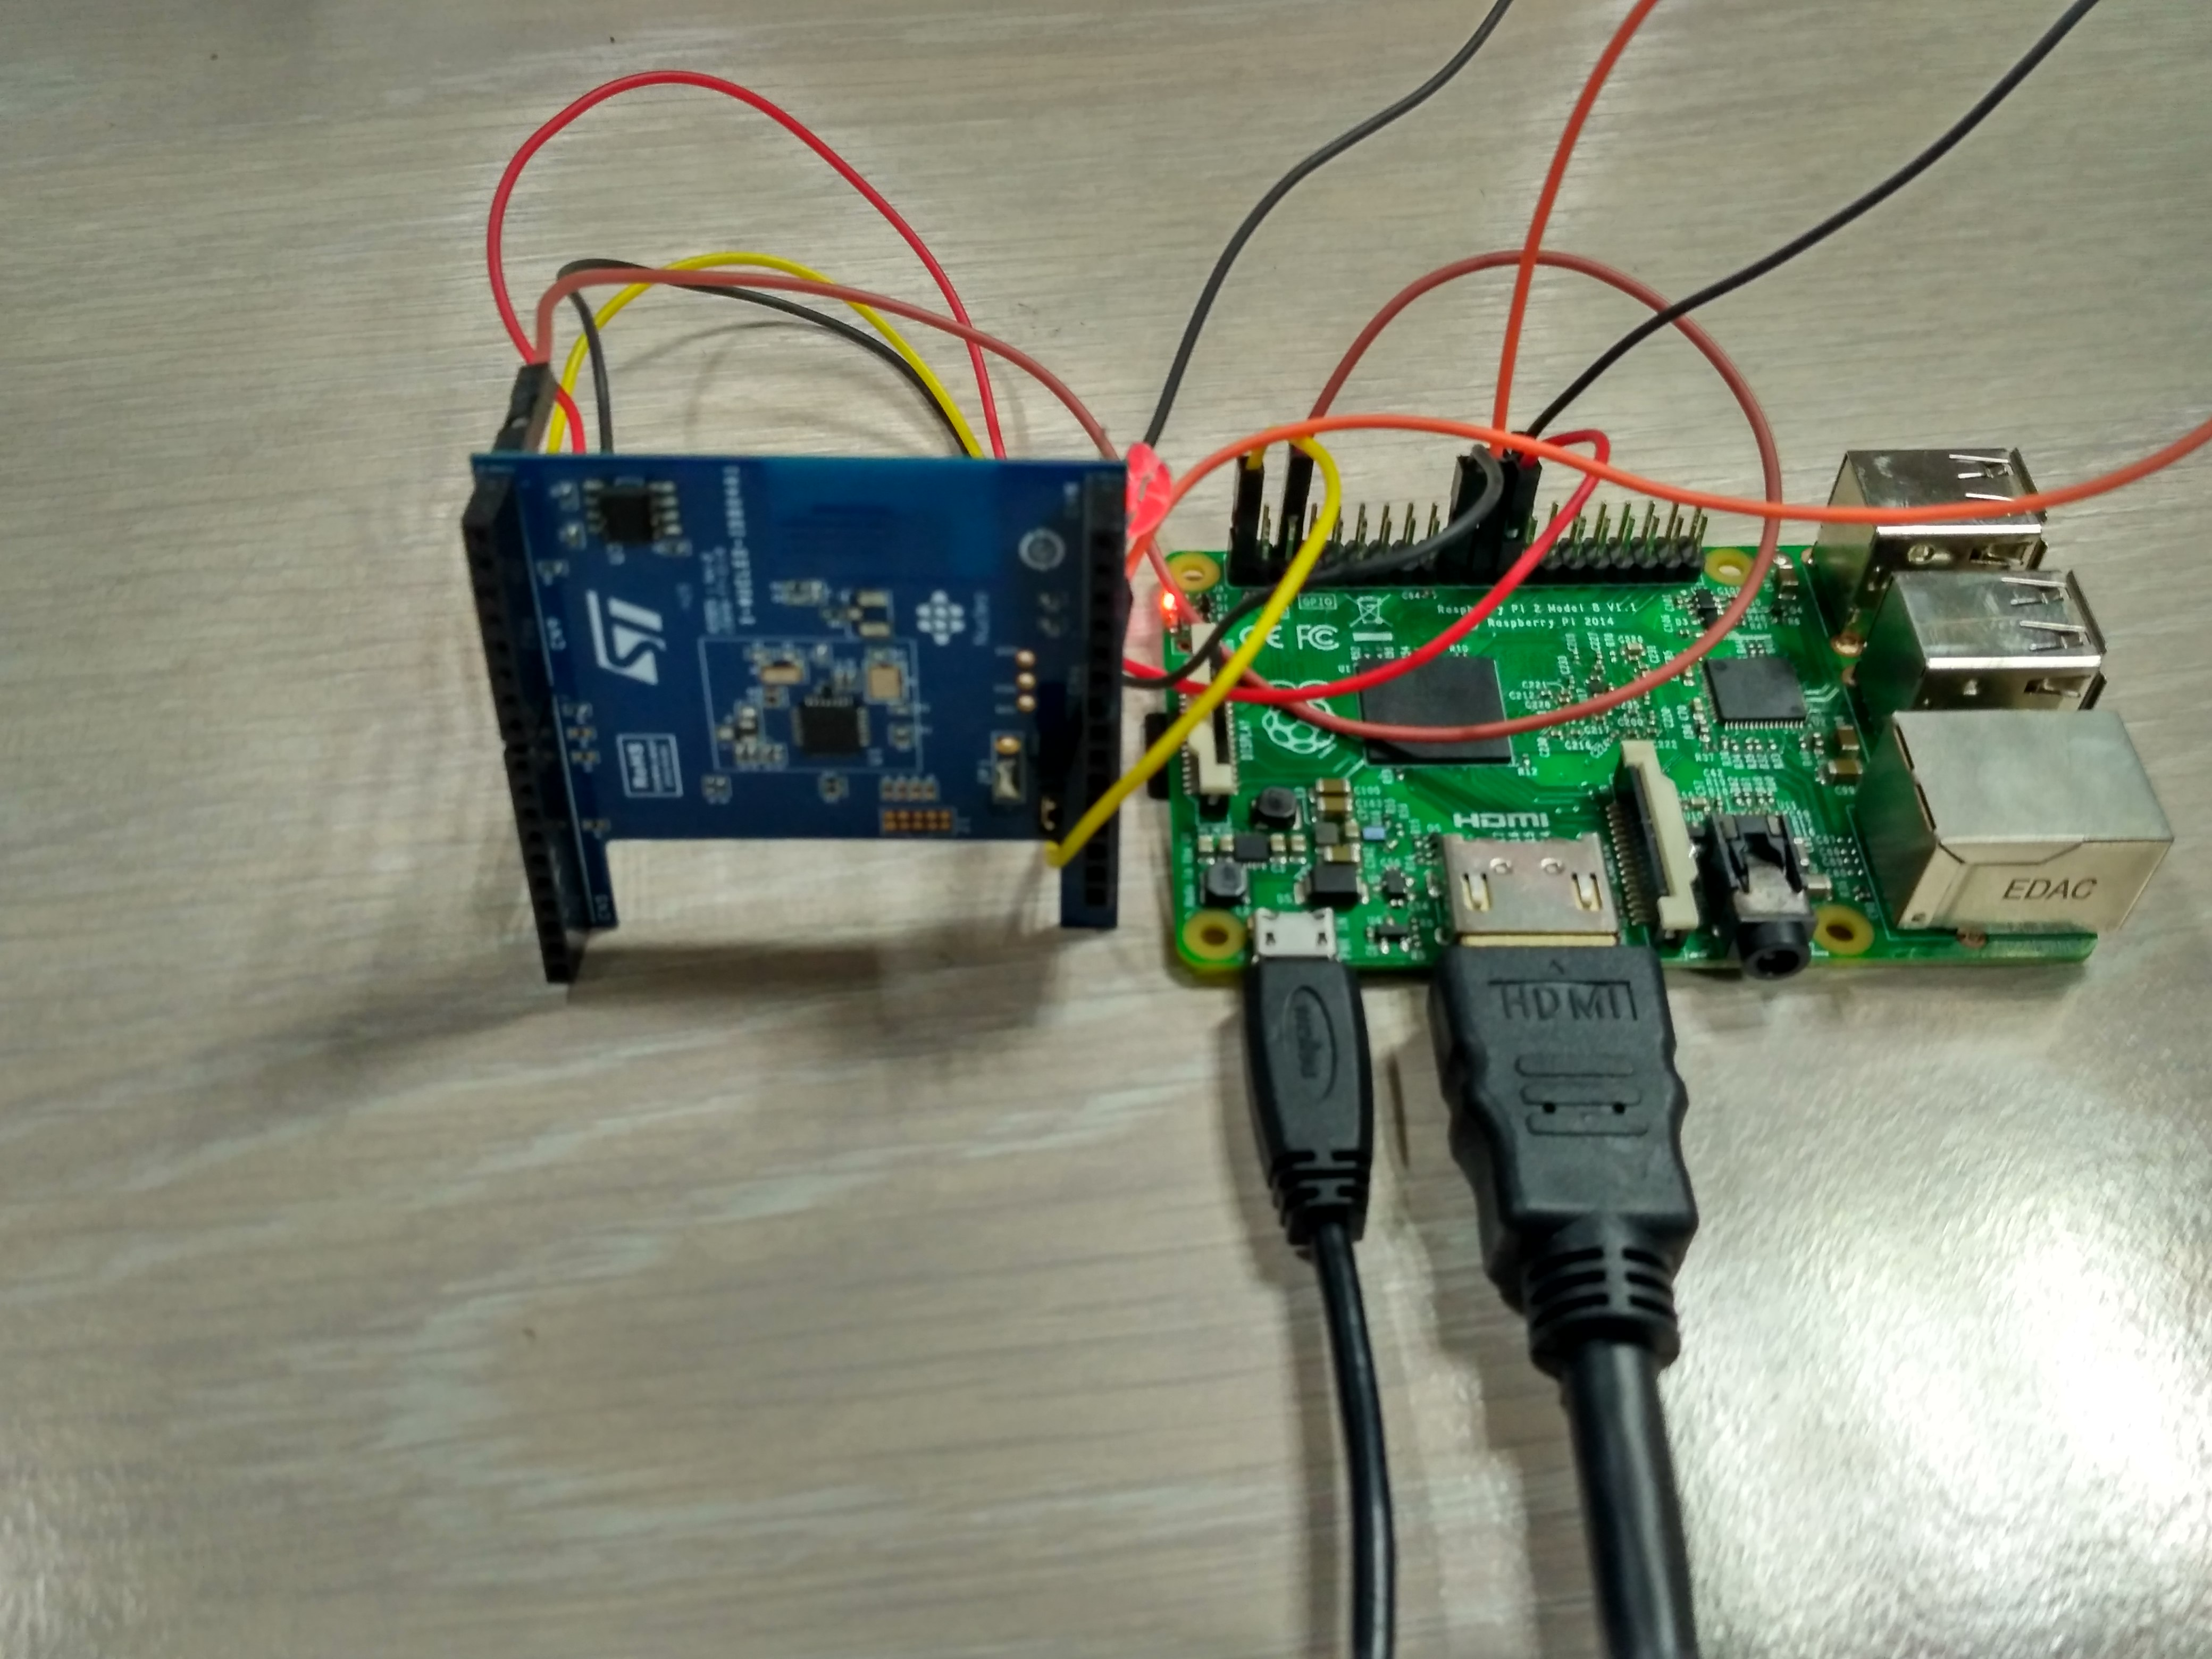
\includegraphics[width=3.5in, height=3in]{images/rpi_connections.jpg}
		\caption{SPI connections}
	\end{figure}
	\item The last step in the implementation is checking to see if the BlueNRG is recognised as an adapter by the Linux kernel. This can be done using the following command:
	\begin{center}
		\textbf{sudo hciconfig}\\
	\end{center}
	This should give the following output listing the adapter.
	\begin{figure}[ht]
		\centering
		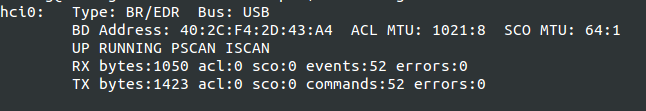
\includegraphics[scale=0.7]{images/adapter_check.png}
		\caption{Checking for adapter}
	\end{figure}
	The adapter can be turned ON and OFF using the following command.
	\begin{center}
		\textbf{sudo hciconfig hci0 on/off}\\
	\end{center}
\end{itemize}
Following the above steps, the working of driver can be tested in the ways described in the \textbf{testing} section of this chapter.
